\chapter{Feats}\label{feats}

There are two basic types of feats. Those that are general and can be taken by anybody, and those that are race specific with the intent on emphasising the unique look and feel that the race contributes to that characters identity. 

\begin{framed}\centering
        On Feat Design. The best kind of feats are those that have really interesting and deep gameplay effects. They should aim to add delicious flavour to the character. They should not rely heavily on some numbers in like +1 in order to deliver impact. 

They do not necessarily have to be mechanical buffs, or even balanced. Some feats are intended to provide players an additional way to make the game for challenging for themselves specifically. Feats that have a fundamental influence on the strategy of a character are also greatly desired as well. 

Feats such as Scholarly Skepticism are designed with the narrative in mind, and they help empower the character to shape the flow of the story. It is thus an explicit declaration to the GM and other players about your character.

The ramification of these design principles can be seen below.           
    \end{framed}

\subsection{General}
    \paragraph{Dead Man Walking} You are living on borrowed time. Do what thou wilt. 
    \paragraph{Haunted} You believe that the spirit of an ally, close friend or something has come back from the grave and now acts as your guardian. This could be a good thing, but it might not be.
    \paragraph{Jaded}
    \paragraph{Redhead} According to folklore, some people born with red hair are marked by the fey. You are one such person. 
    \paragraph{Reincarnated} You have vague, dream-like memories of a past life. You might even possess skills that you never knowingly learned.
    \paragraph{Coward} Upon reaching 40\% of your current health, you automatically flee as soon as possible.
    \paragraph{Hardened Criminal}
    \paragraph{Seasoned Traveller} This feat can be gained for free by sufficiently exploring the world. 
    \paragraph{University Education}
    \paragraph{Albino}
    \paragraph{Machiavellian} You have a silver tongue and a natural presence about you. You have learned to put this innate charm to use as a political predator. 
    \paragraph{Vampirism} Your max health is halved. In exchange, you can lifesteal.
    \paragraph{Scholarly Skepticism} You possess a keen logical mind and put faith only in your rationality and observation. 
    \paragraph{Portents} You are blessed (or cursed) with hazy visions of the near future. These take the form of vague feelings of comfort or dread that manifest on the cusp of pivotal choices. 
    \paragraph{Smitten} You are truly and deeply in love, in the purest storybook sense. Your love is not necessarily requited, but acts as a source of strength and purpose, for you would cross oceans and mountains to protect your beloved. 
    \paragraph{Military Veteran}
    \paragraph{Damned} For some reason a God has marked you down as undesirable. The reason is up to you. 
    \paragraph{Innocent}
    \paragraph{Unyielding Devotion} So firm are you in your crusade that your mind is nearly unassailable by those who would end it. Your faith literally dominates your life. Heresy hits you with feelings of rage and indignation, compelling you to ruthlessly stamp it out. So strong is your belief in the righteousness of your struggle that you inspire others by your example. 
    \paragraph{Paranoid} Self explanatory. Sometimes your belief might be unfounded or exaggerated. But those odd times when you are right, you will be glad you are a paranoid bastard.
    \paragraph{Forsaken Thoughts} The origin of the meditations of the Forsaken Thoughts is shrouded in secrecy. No warrior has ever admitted to knowing them, for the techniques were said to involve rejecting the Divine in all its forms.
\subsection{Flaws}
    \paragraph{Near-sighted} Things far away seem blurry.
    \paragraph{Braggart} You tend to EXAGGERATE!
    \paragraph{Eidetic Memory} You tend to remember things with absolute clerity.
    \paragraph{Alzheimers} You have trouble remembering where you are. You are not allowed to use any maps.
    \paragraph{Know No Pain} You dont know your HP. 
    \paragraph{Tunnel Vision} You often lack peripheral vision. 
    \begin{figure}[h]
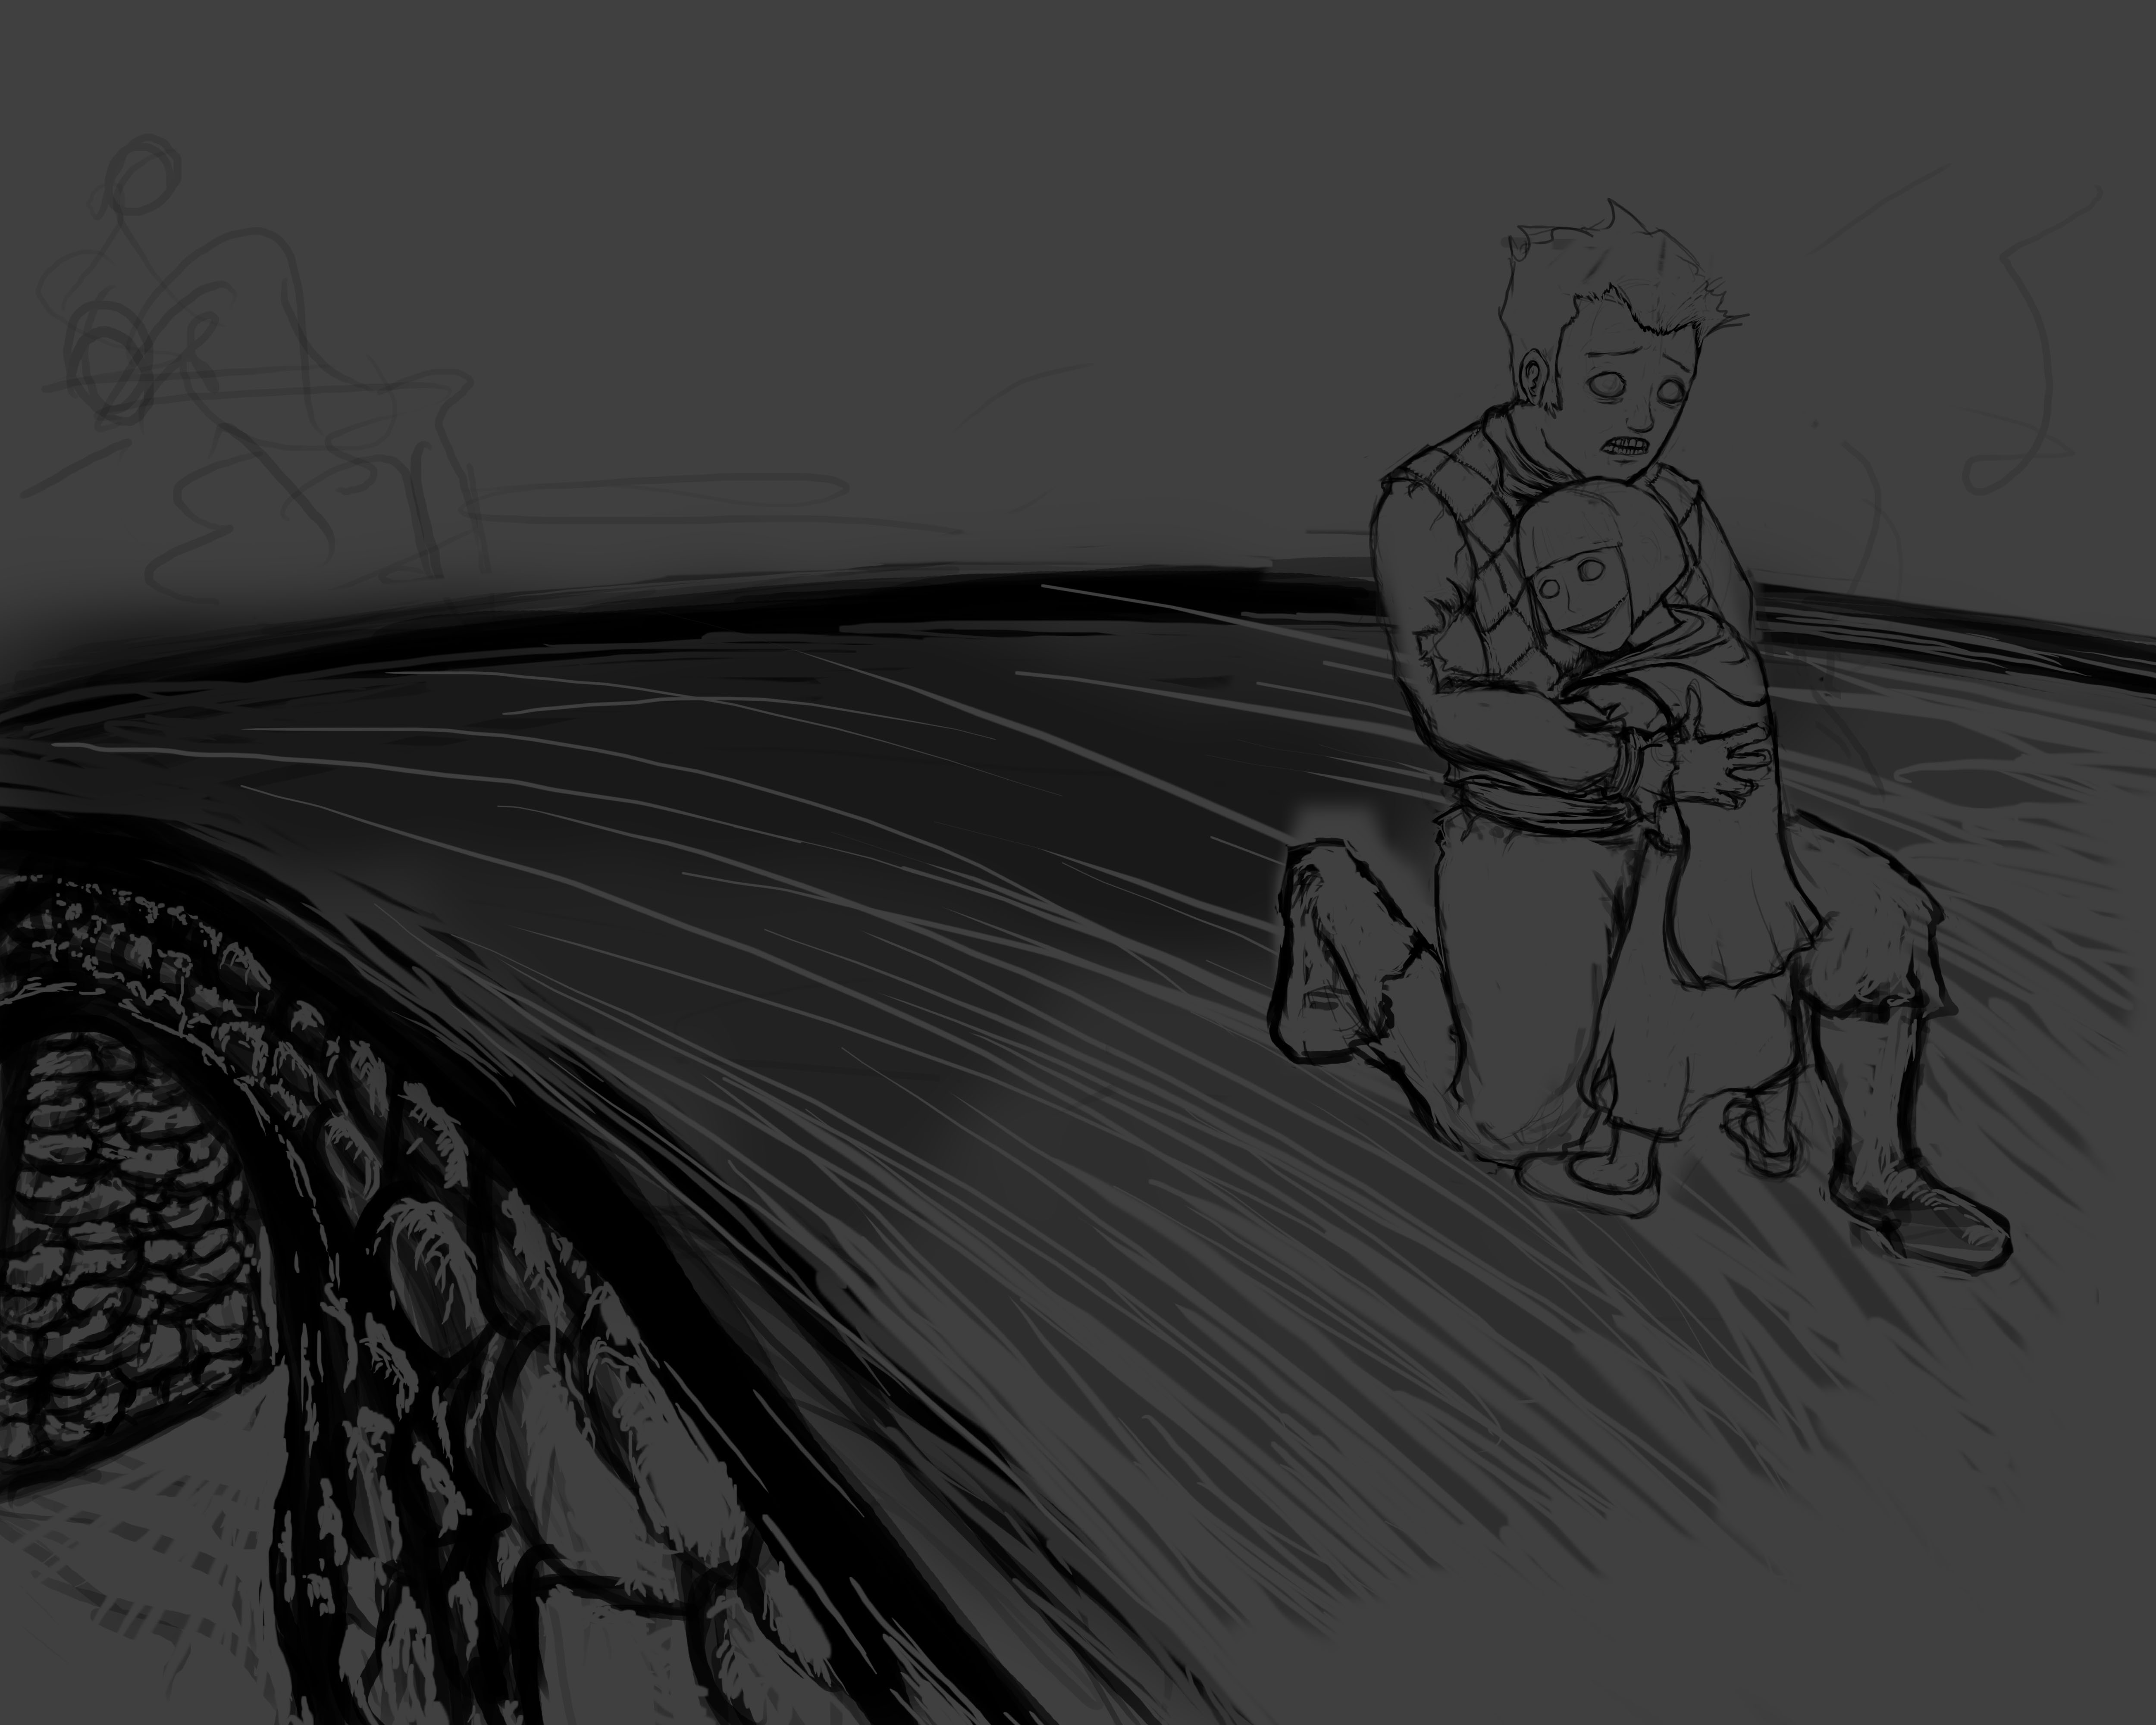
\includegraphics[width=\columnwidth]{rakaarth4}
\end{figure}
\subsection{Racial - Fire Giant}
    \paragraph{Heart of Fire} You are immune to any form of fire damage.
    \paragraph{Door Smasher} You can smash down a wooden door in a single round (6 seconds). 
\subsection{Racial - Gnoll}
    \paragraph{Refuse Eater} You gain sustenance from, and are resilient to, foods that would be considered disgusting by other Races standards. 
    \paragraph{The Hunt} Gnolls with this feat are the best at punishing foes who flee a close quarter engagement. I suggest allowing for a free attack.    
\subsection{Racial - Human}
    \paragraph{Outlander} You are literally not from this world. Outlanders simply appear in the wilderness with no gear at all. Unless an outlander actively aims to culturally immerse themselves they always seem to be foreign to the locals - in part because of their appearance, mannerisms, accent and behaviour. Except in the most cosmopolitan of areas, Outlanders are seen with at least suspicion, if not worse.
\subsection{Racial - Wood Elves}
    \paragraph{Woodland Traveller} Forest type terrain causes you no movement penalties.
    \paragraph{Squirrel} Fleeing a close quarter engagement is much less dangerous for you.
    \paragraph{At Peace with Nature} All natural wildlife are passive towards you and begin with the neutral mentality. One consequence of this is that even the most cowardly of animals will not flee on discovering your presence. 
    \begin{framed}\centering
        The Gnoll race are the best Hunters and the Wood Elf race are the best at escaping combat. Both their racial feats cancel each other out - and thus fleeing and chasing is as normal. Thus, they counter each other in a sense.          
    \end{framed}
\subsection{Racial - Dark Elf}
    \paragraph{Improved Infravision} Doubles infravision range to 120ft.
    \paragraph{Climb Steep Surfaces} They can climb as a rogue. If they are a rogue, they climb twice as fast as normal. A consequence of this is that Dark Elves are capable of taking advantage of certain terrain in ways that other races are simply not capable of doing so.
\subsection{Racial - Dwarf}
    \paragraph{Unyielding before Death} Dwarves whom reach the state when others die instead get forced into a catatonic coma state. This occurs unless the Dwarf dies to massive damage. If the Dwarf suffer further damage - such as being executed - they will die. After a time period, such as 1 week, the Dwarf will recover to 0 hp.  
    \paragraph{Dwarven Vigor} You heal health at twice the normal rate. 
    \paragraph{Vengeance Seeker} It is a terrible idea to wrong a Dwarf for they have deep memories, long lifespans, and a thirst for vengeance that eclipses most men. Dwarves are capable of memorising the faces of those whom wronged them to the most minute detail - an almost picture perfect memory - and this image haunts them till the day they die. A consequence of this is that it aids the Dwarf in hunting down those whom have provoked their wrath. 
\subsection{Racial - Gnome} 
    \paragraph{Family Connections}
\subsection{Racial - Half Elf} 
    \paragraph{Stars in the Night Sky} Many Half Elves are extremely extroverted, and more than any other race capable of building and developing relationships and reputations with people. Half Elves are allowed one additional Henchmen above what is ordinarily allowed just due to their force of personality. Additionally, once per day when dealing with any problem, a Half Elf may declare that they know someone who could help the players in this problem; it is upto the players and the GM to determine who could feasibly help, and importantly, how will they know and how will they get there. 